\documentclass[14ppt]{article}
\usepackage[utf8]{inputenc}
\usepackage{amsmath}
\usepackage{amsfonts}
\usepackage{graphicx}
\usepackage[colorinlistoftodos]{todonotes}
\usepackage[Algoritm]{algorithm}
\usepackage[noend]{algpseudocode}
\usepackage{txfonts}
\usepackage{url}
\usepackage{hyperref}
\usepackage{geometry}
\newcommand\tab[1][1cm]{\hspace*{#1}}
\begin{document}
\begin{titlepage}
    \begin{center}
    \Large
        University of Craiova\\
        Faculty of Automation, Computers and Electronics\\
         
\includegraphics[width=0.2\textwidth]{ace.png}
        \vspace*{2cm}
            
        \Huge{\textbf{Dijkstra}\\}
        \vspace{0.3cm}
        \Large
        Parallel and Distributed Algorithms
            
        \vspace{1.5cm}
            
        \Large \textbf{Student}\\ Smarandache Alexandru
        \\\vspace{0.25cm}
        \Large{\textbf{Computers Romanian Language }}\\
        \Large{Study Group CR 3.2}\\
         \Large{\textbf{Third Year}}\\
        \vfill
    
        \vspace{0.8cm}
            
        \Large
        March 2022
    \end{center}
\end{titlepage}
\begin{center}
\tableofcontents
\end{center}

\newpage
\section{Implementations of Dijkstra's algorithm}
\subsection{C++ Sequential}
\subsection{Java Sequential(using priority queue)}
\subsection{C++ STL parallel}
\subsection{C++ OpenMP}
\subsection{C++ MPI}
\subsection{Java Parallel Streams}
\subsection{Java with Threads}
\vspace{1cm}
\section{Input data generation}
To generate input data, a graph is generated based on a given density.\\
Input format:\\
noOfNodes sourceNode\\
c00 c01 ... c0(noOfNodes -1)\\
c01 c11 ... c1(noOfNodes -1)\\
...\\
c(noOfNodes -1)0 c(noOfNodes -1)1 ... c(noOfNodes -1)(noOfNodes -1) \\\\
Where:
\begin{itemize}
    \item \textbf{noOfNodes}: the number of nodes
    \item \textbf{sourceNode}: the source node 
    \item \textbf{c}: the adjacency matrix
\end{itemize}
\begin{center}
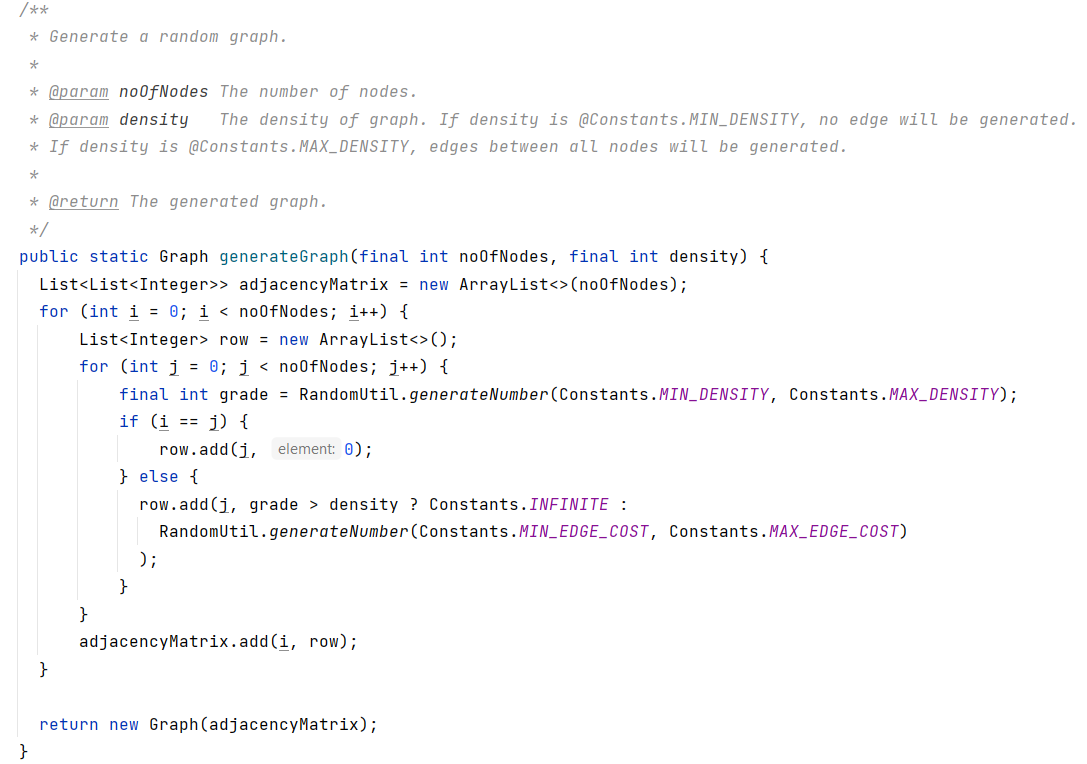
\includegraphics[ width = 17cm]{data_generation_code.png}
\end{center} 
\section{Output data}
Each algorithm will have the following output format:\\
Vertex 	Distance from source(source node)\\
0       c0\\
1       c1\\
...\\
noOfNodes -1 c(noOfNodes - 1)\\
Where:\\
c[i] is the distance between node i and source node.
\newpage
\section{Results}
\subsection{C++ Sequential}
\begin{center}
\includegraphics[ width = 15cm]{c++_seq.png}
\end{center} 
\subsection{Java Sequential(using priority queue)}
\begin{center}
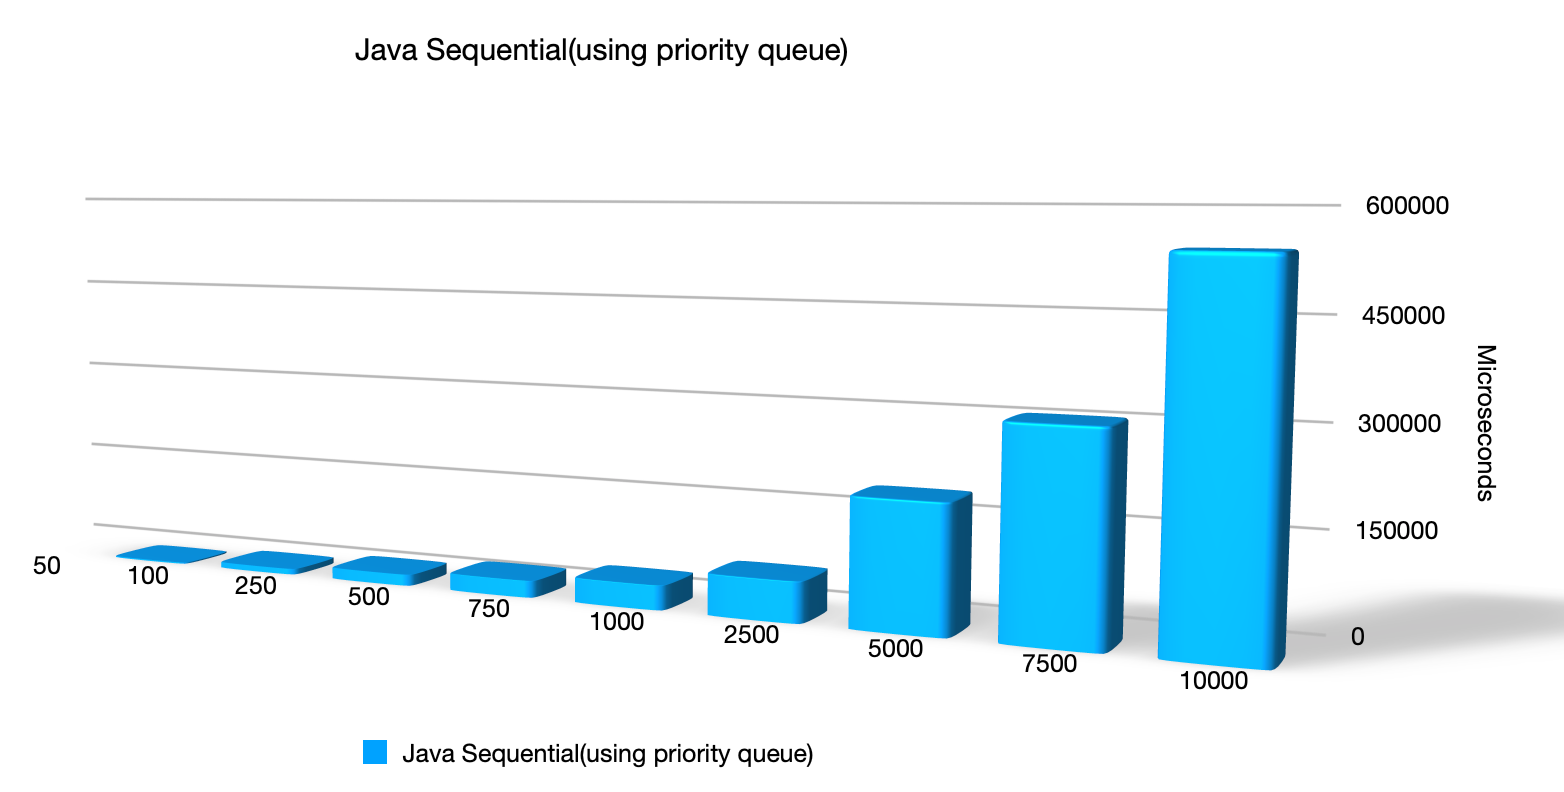
\includegraphics[ width = 15cm]{Java_seq.png}
\end{center} 
\subsection{C++ STL parallel}
\begin{center}
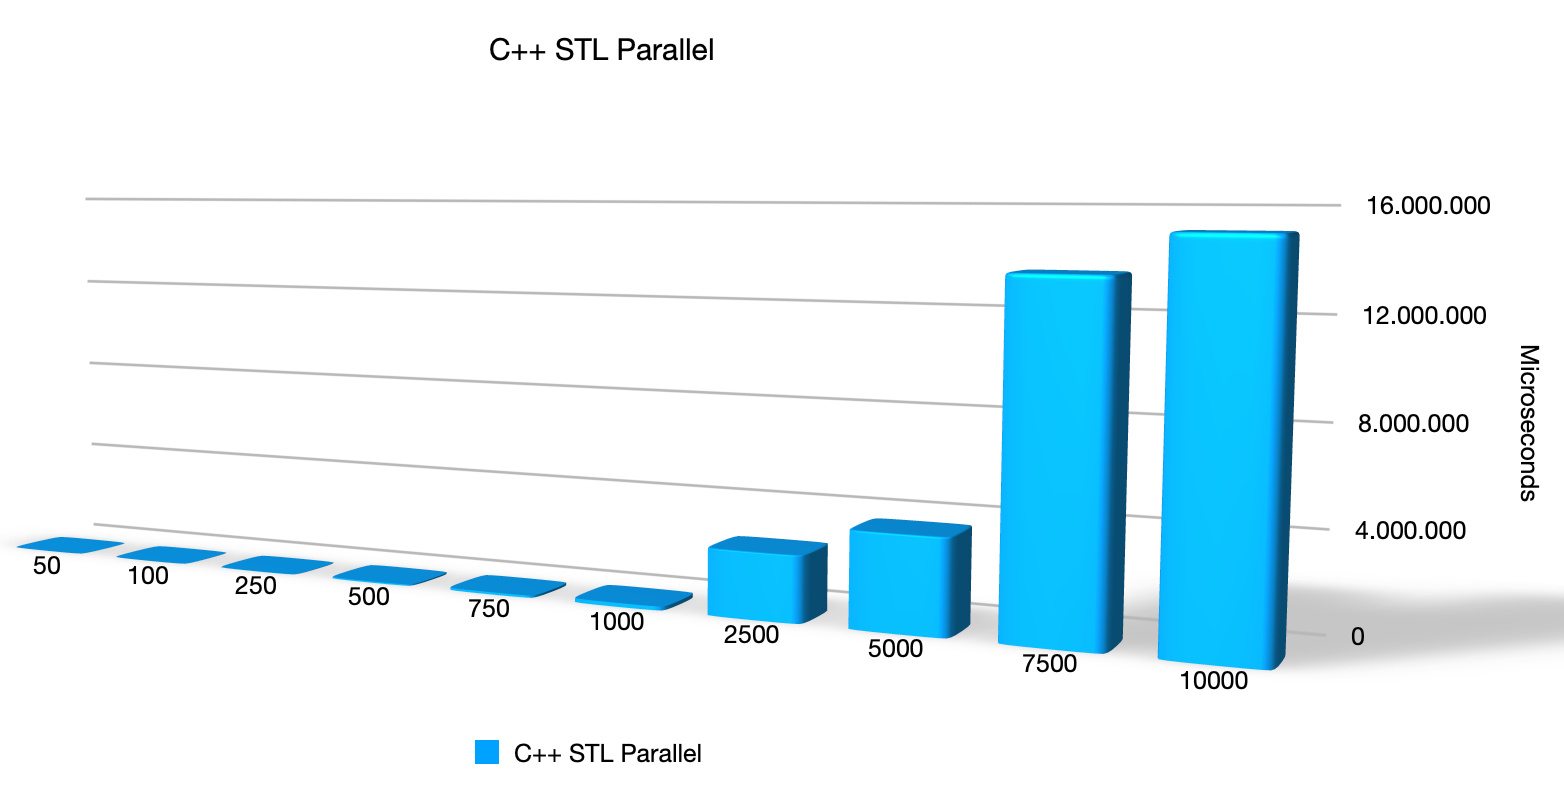
\includegraphics[ width = 15cm]{C++_stl_par.png}
\end{center} 
\subsection{C++ OpenMP}
\begin{center}
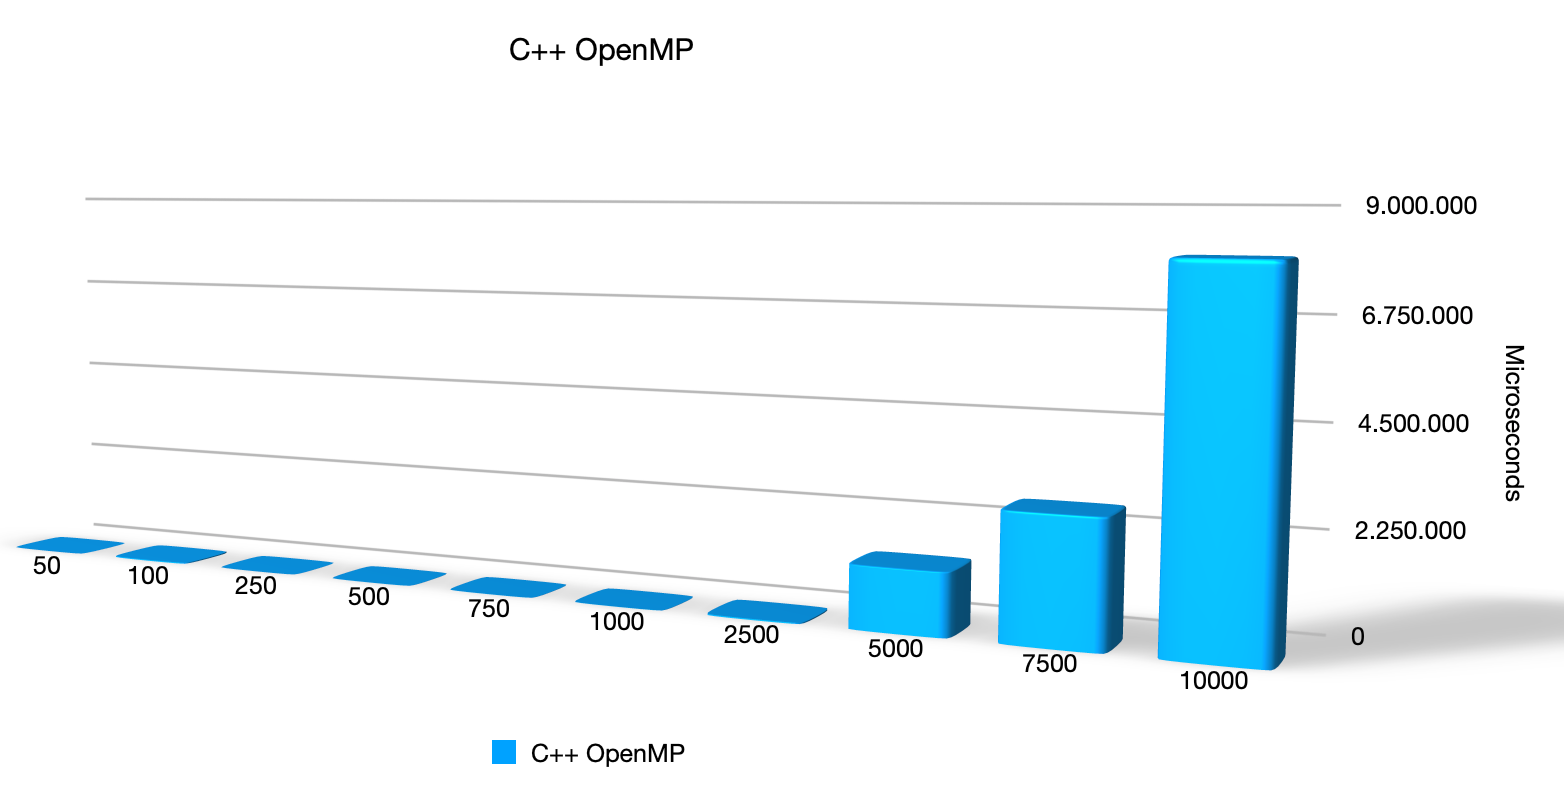
\includegraphics[ width = 15cm]{C++_OpenMP.png}
\end{center} 
\subsection{C++ MPI}
\begin{center}
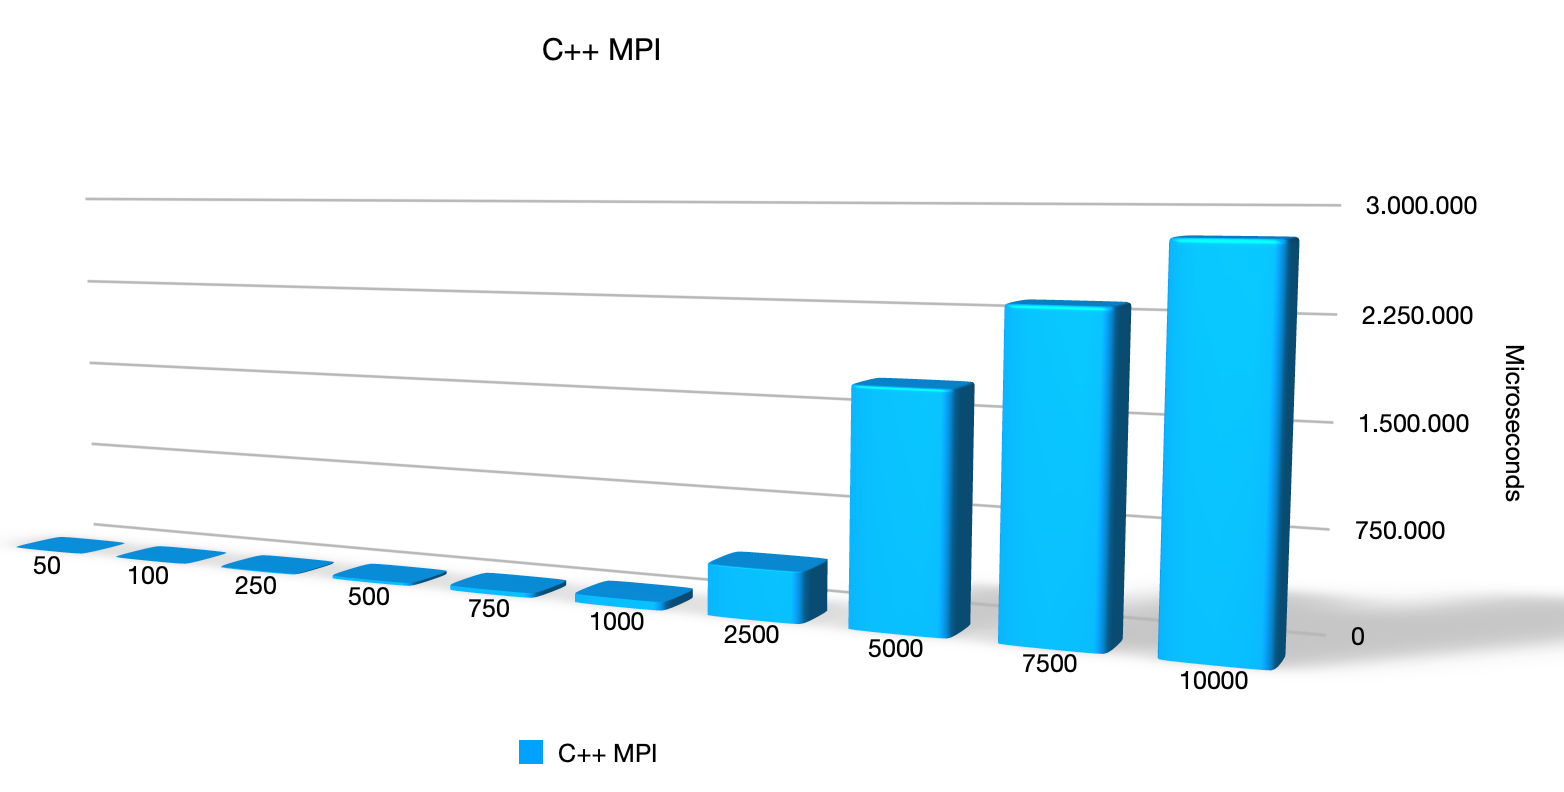
\includegraphics[ width = 15cm]{C++_MPI.png}
\end{center} 
\subsection{Java Parallel Streams}
\begin{center}
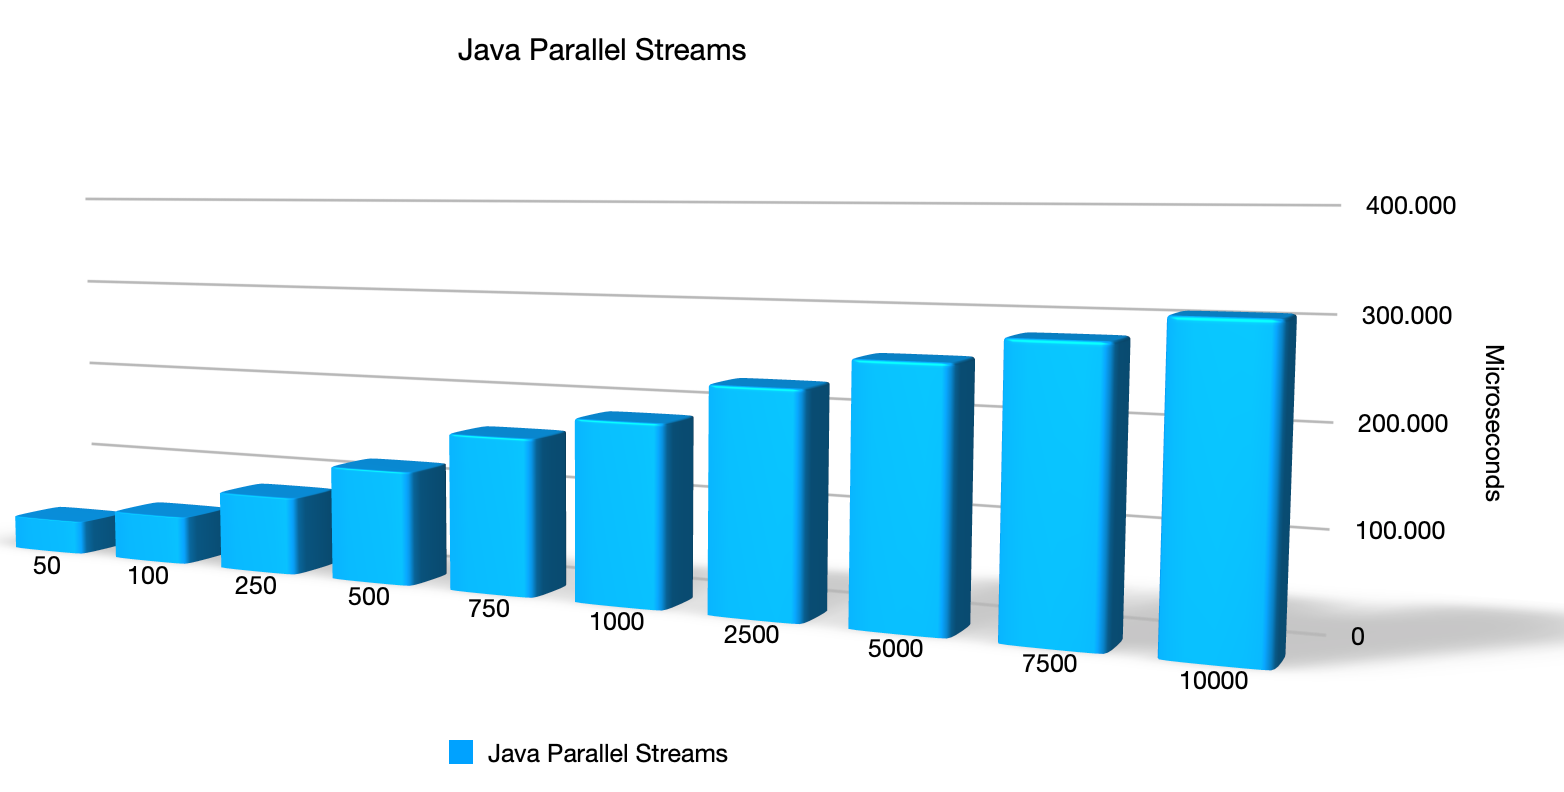
\includegraphics[ width = 15cm]{Java_Streams.png}
\end{center} 
\subsection{Java with Threads}
\begin{center}
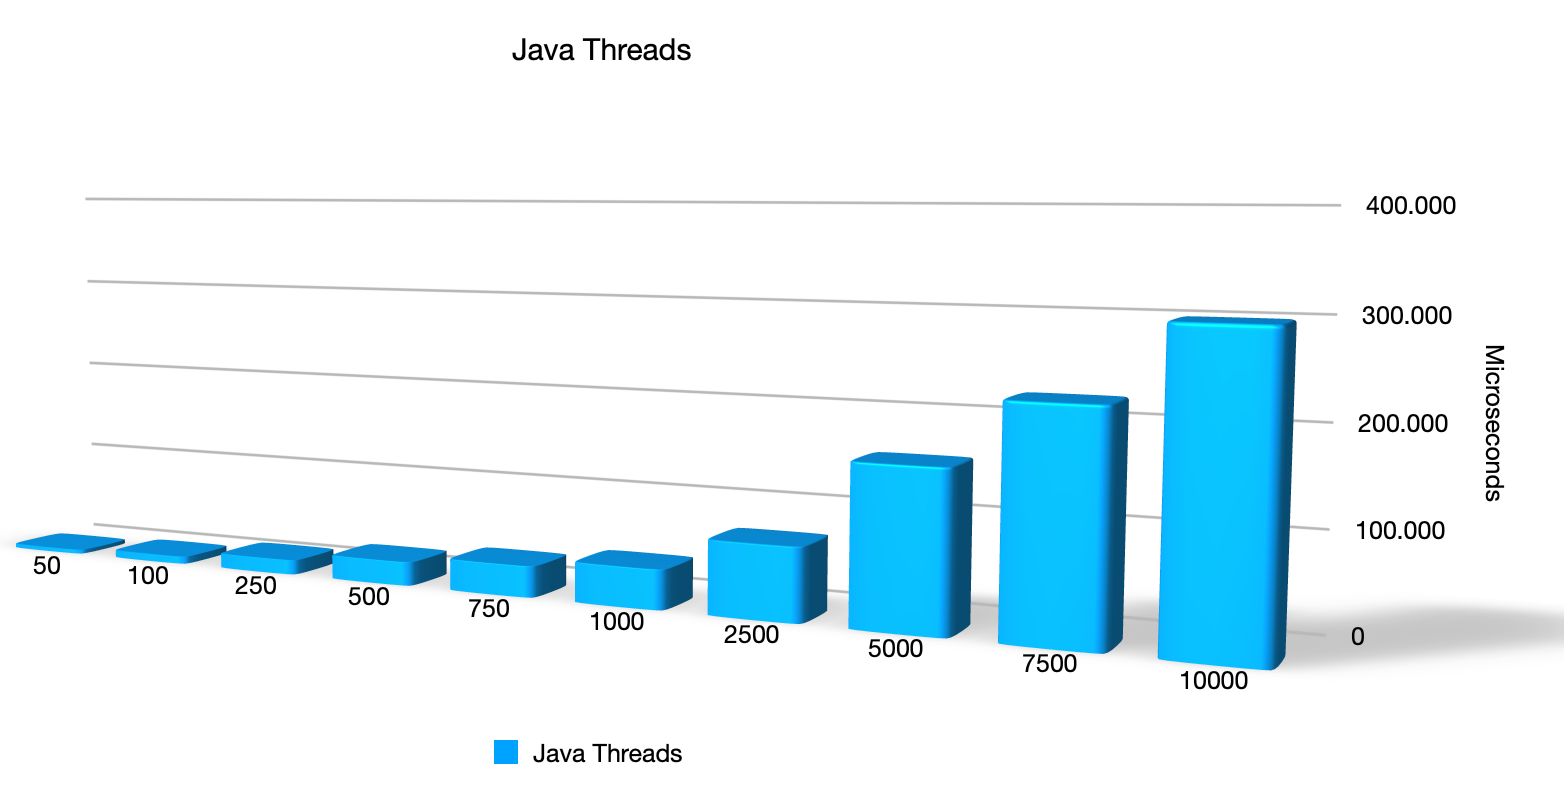
\includegraphics[ width = 15cm]{Java_Threads.png}
\end{center} 
\newpage
\section{Comparasion}
\subsection{All implementations}
\begin{center}
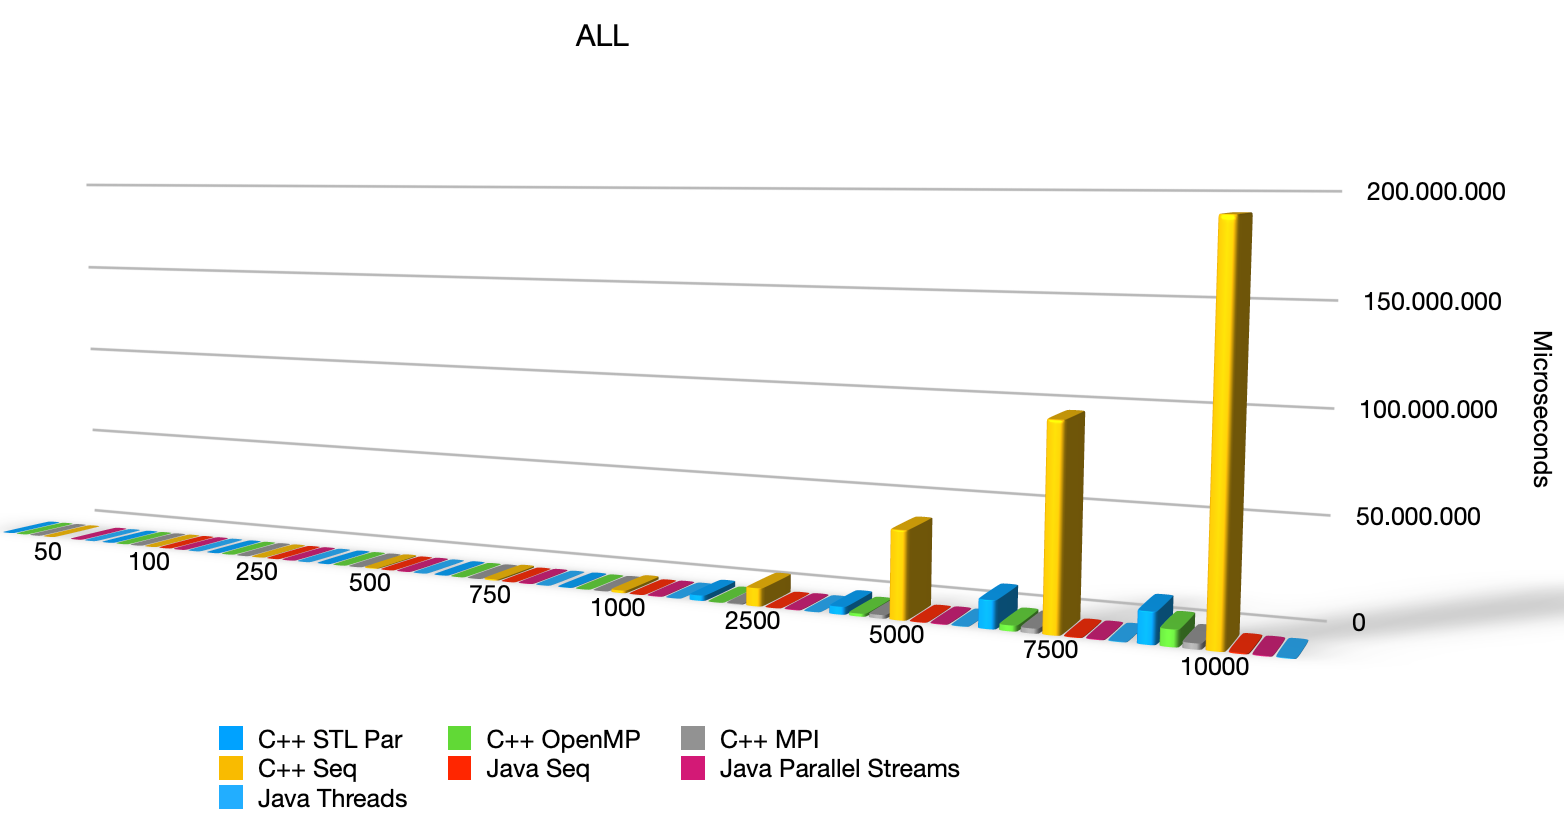
\includegraphics[ width = 15cm]{All.png}
\end{center} 
\subsection{C++ implementations}
\begin{center}
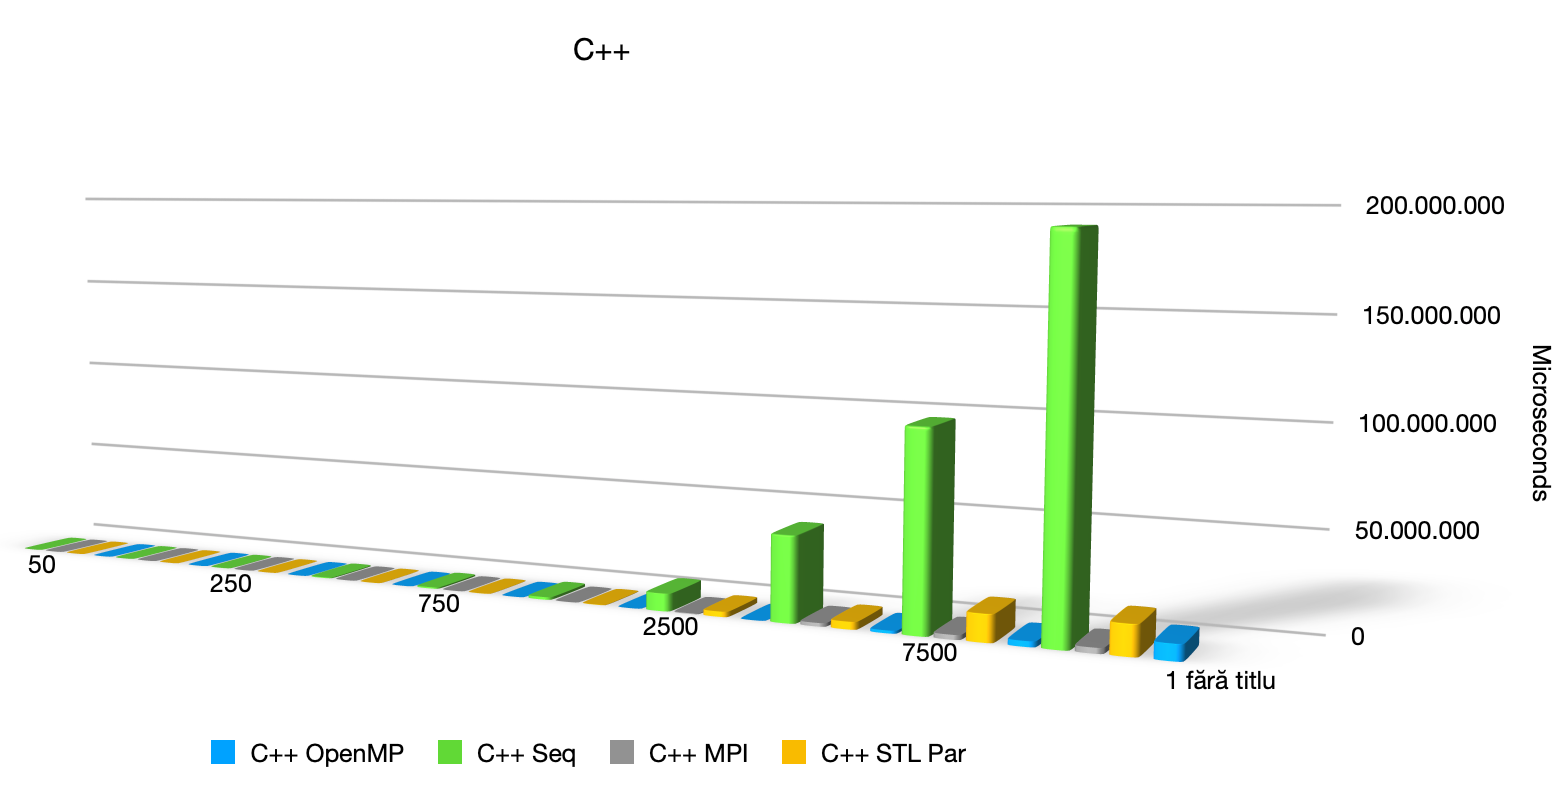
\includegraphics[ width = 15cm]{C++_All.png}
\end{center} 
\subsection{Java implementations}
\begin{center}
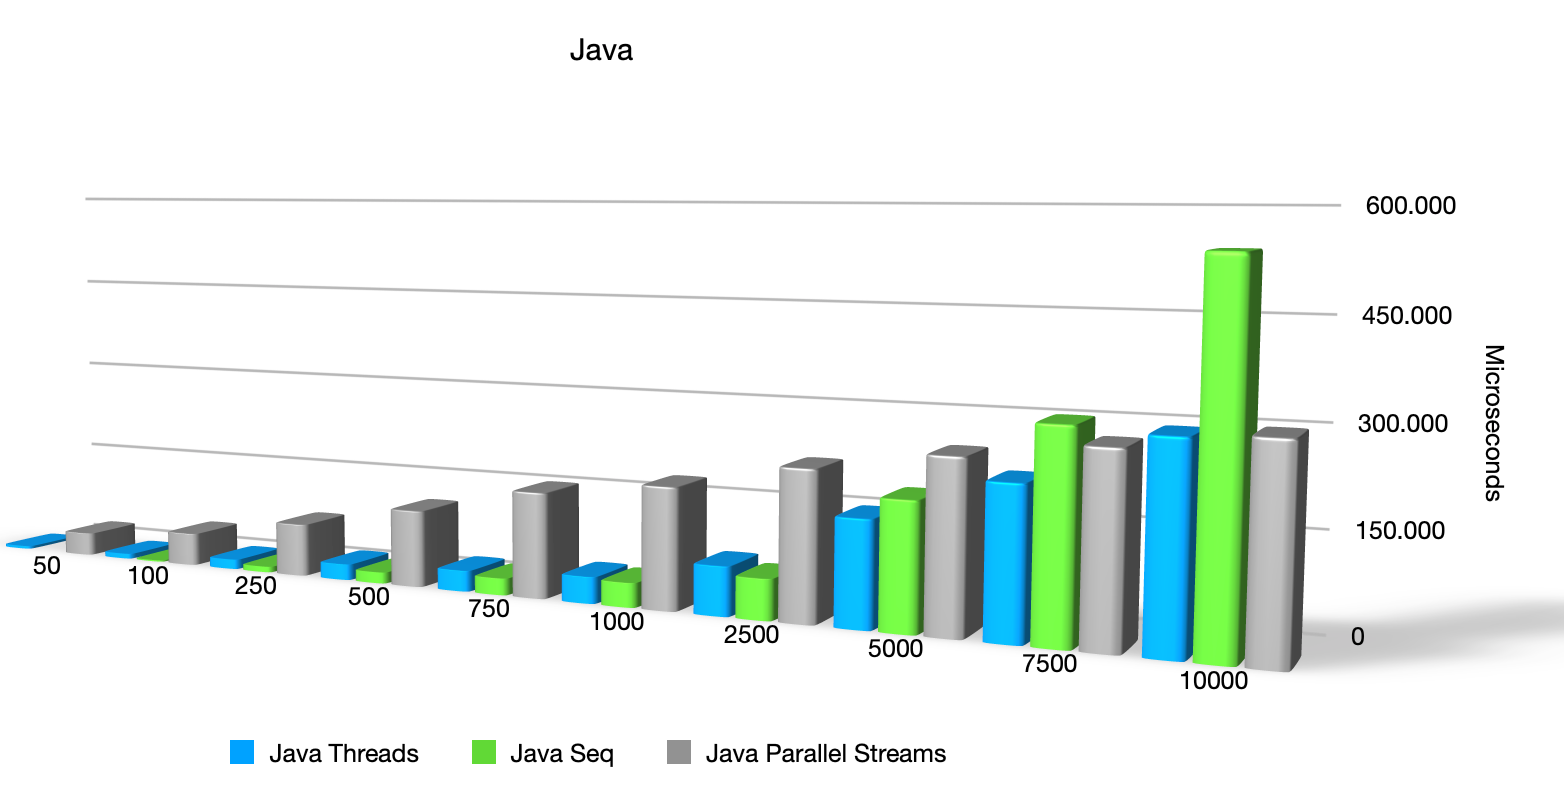
\includegraphics[ width = 15cm]{Java_All.png}
\end{center} 
\subsection{C++ STL Parallel vs Java Streams Parallel}
\begin{center}
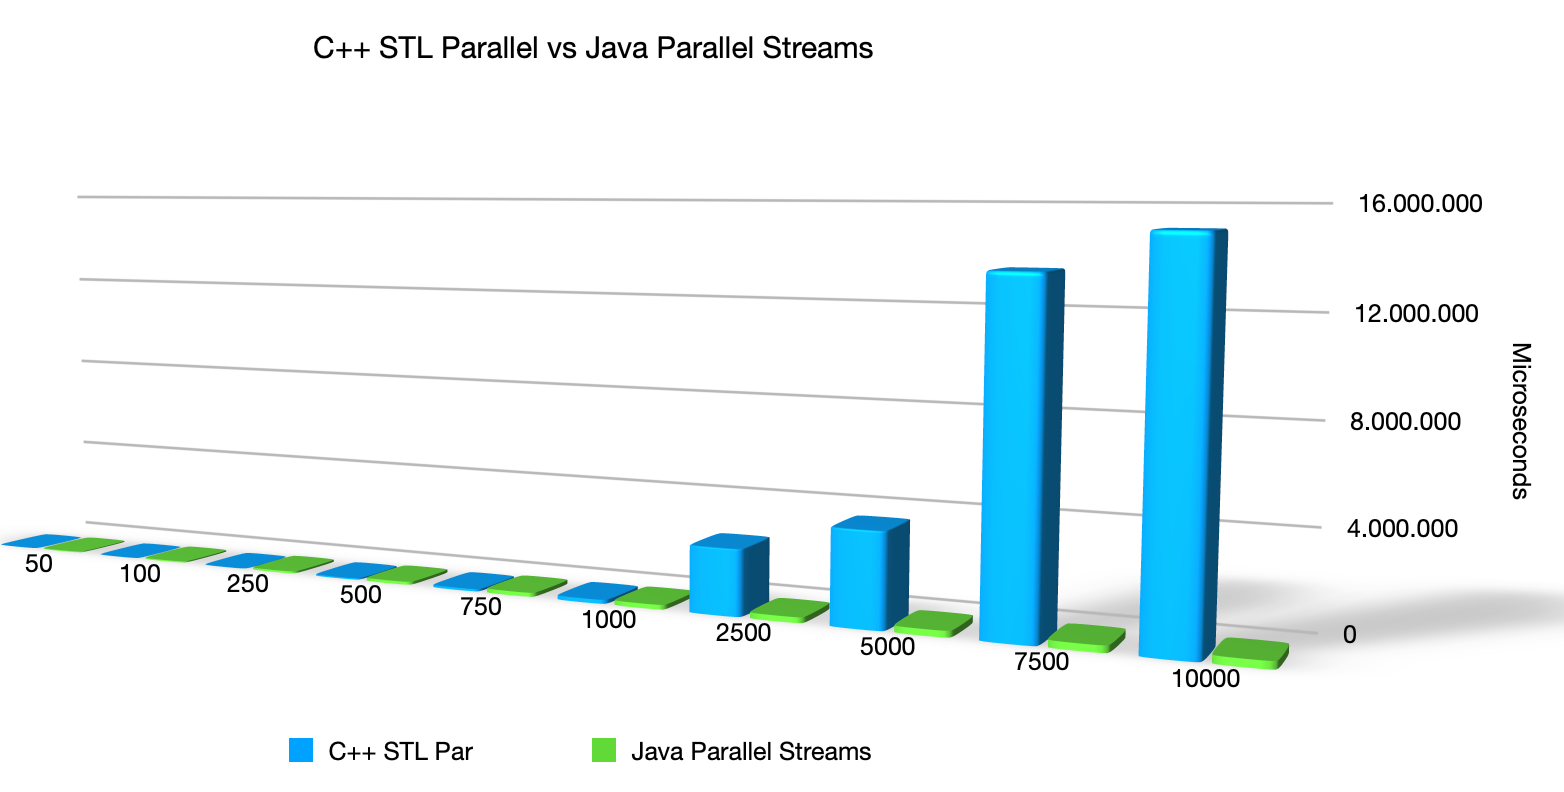
\includegraphics[ width = 15cm]{C++_STL_vs_Java_Streams.png}
\end{center} 
\subsection{C++ Parallel}
\begin{center}
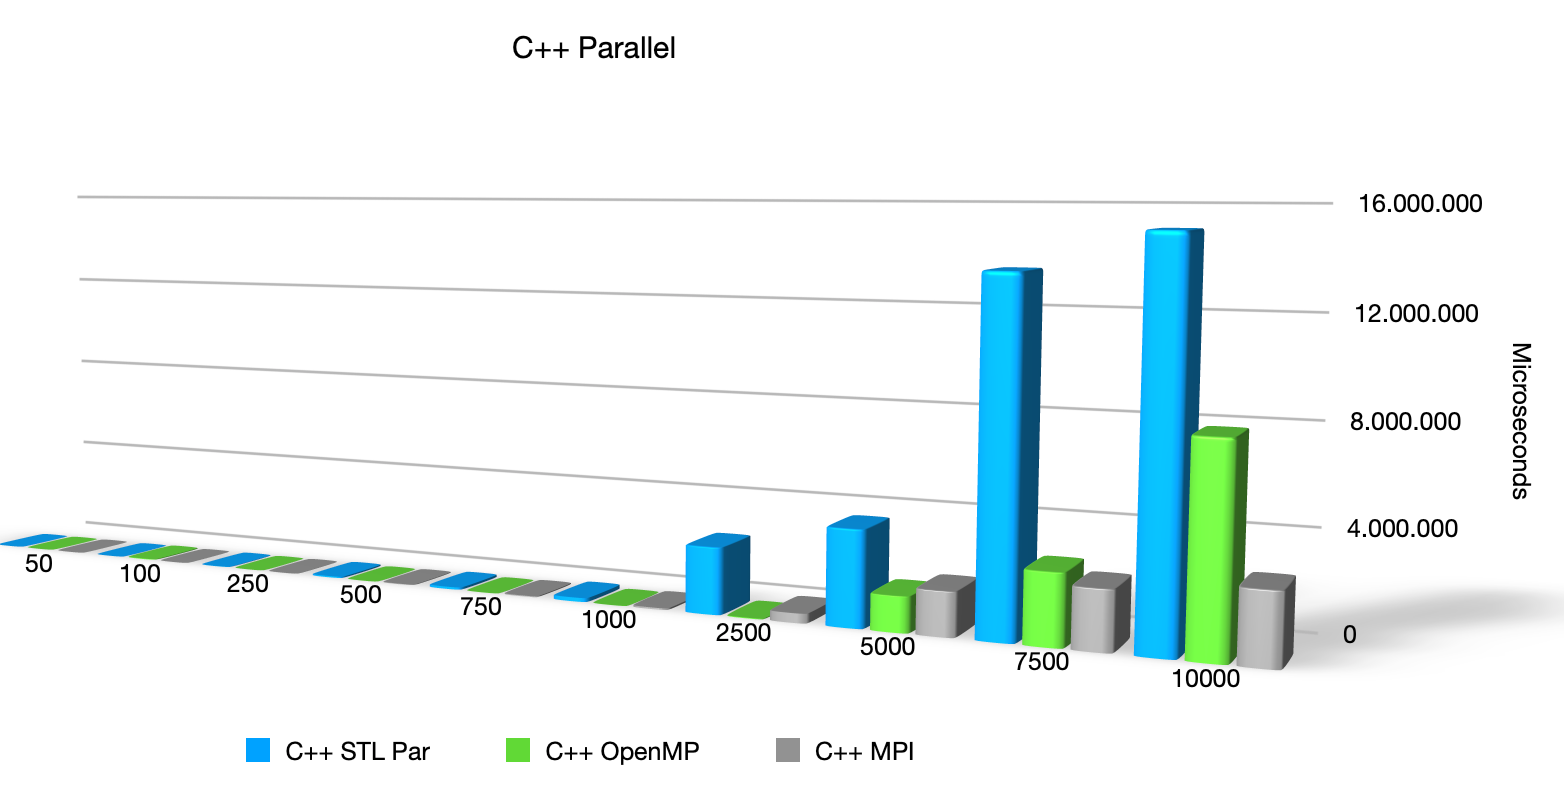
\includegraphics[ width = 15cm]{C++_Parallel.png}
\end{center} 
\textbf{Observation}\\
The environment on which I ran the tests is: Windows 10 Home, 16GB Ram, 512GB SSD, Eclipse for Java programs and Visual Studio 2019 for C++.
\newpage
\section{Bibliography}
\begin{thebibliography}{9}

    \bibitem{repository.stcloudstate.ed}
     repository.stcloudstate.ed,\url{https://repository.stcloudstate.edu/cgi/viewcontent.cgi?article=1044&context=csit_etds}, accessed in March 2022.

    \bibitem{geeksforgeeks}
     geeksforgeeks,\url{https://www.geeksforgeeks.org/dijkstras-shortest-path-algorithm-greedy-algo-7/},
     accessed in March 2022.
\end{thebibliography}
\end{document}
